% \section{第4讲\quad 应用题}

\item {
    【归一问题】
    一筐水果中, 恰好有一半数量是苹果,如果吃掉苹果数量的一半, 筐中只剩下 60 个水果,那么,这时筐子中还有\underline{\hbox to 20mm{}}个苹果.
    \ifshowSolution{}
        \fangsong\zihao{5}\textcolor{blue}{
            \\正解:\\
            假设原来苹果有2份,则另一种水果也是2份。\\
            吃掉1份苹果后,筐中还剩下3份,所以,一份水果是
            \[
                60\div 3 = 20个.
            \]
            所以,这时筐子中还有 20个苹果.
        }
    \else
        \vspace{2cm}
    \fi
    % 2021;迎春杯四年级真题.pdf; 20
}

\item {
    【火车过桥】
    一个车队以4米/秒的速度缓慢通过一座长298米的大桥,共用115秒,已知每辆车长6米,相临两车间隔20米,则这个车队一共有 \underline{\hbox to 20mm{}} 辆车.
    \ifshowSolution{}
        \fangsong\zihao{5}\textcolor{blue}{
            \\正解:\\
            车队长:\[115\times 4﹣298=162 (米), \]
            车的间隔数是:\[(162﹣6)\div (20+6)=6(个),\]
            车一共有:\[ 6+1 = 7(辆).\]
        }
    \else
        \vspace{2cm}
    \fi
    % 2012年第十七届“华罗庚金杯”少年数学邀请赛决赛试卷(小中组a卷), 7
}

\item {
    【平均数】
    某旅行团由6位男士和9位女士组成.已知6位男士的平均年龄是57岁9位女士的平均年龄是 52 岁.则这个旅行团所有成员的平均年龄是 \underline{\hbox to 20mm{}}岁.
    \ifshowSolution{}
        \fangsong\zihao{5}\textcolor{blue}{
            \\正解:\\
            \[(6\times 57 + 9\times 52)\div (6+9)=54.\]
        }
    \else
        \vspace{2cm}
    \fi
    % 2022.2.19线上小中组解析1.pdf;54
}

\item {
    【鸡兔同笼】
    鸡兔关在同一个笼子里, 鸡比兔子少20只. 兔脚的数量比鸡脚的数量的3倍多10只.那么鸡有\underline{\hbox to 20mm{}}只. 
    \ifshowSolution{}
        \fangsong\zihao{5}\textcolor{blue}{
            \\正解:\\
            设鸡有x只,则兔有x+20只.
            \[2x\cdot 3 + 10 = 4(x+20)\]
            \[x = 35.\]
        }
    \else
        \vspace{2cm}
    \fi
    % 2020华数之星初赛-三四年级真题.pdf; 35
}

\item {
    【鸡兔同笼·倒扣问题】
    工人运瓷器 1000件, 规定完整运到目的地一件给运费5元, 损坏一件倒赔120 元;运完这批瓷器后,工人共得 4500元, 那么损坏了 \underline{\hbox to 20mm{}}件.
    \ifshowSolution{}
        \fangsong\zihao{5}\textcolor{blue}{
            \\正解:\\
            假设1000件瓷器都是完好运送,则应得\\
            \[1000\times 5 = 5000(元)\]
            实际差额: 
            \[5000-4500=500(元).\] \\
            由于一件被损坏的产品被假设成完好运送会多加:
            \[120+5=125(元)\]
            所以损坏的数量:
            \[500\div 125 = 4(件).\]
        }
    \else
        \vspace{2cm}
    \fi
    % 2023YCB原题小中组(1).pdf;4
}

\item {
    【还原问题】
    暑假期间小明在家写字.第一天写了比总字数的一半还少 50个的字, 第二天写了余下字数的一半还少 20 个字, 第三天写了再余下字数的一半多 10个字, 第四天写了 60 个字, 还剩 40 个字就全部写完了:小明假期一共要写\underline{\hbox to 20mm{}}个字.
    \ifshowSolution{}
        \fangsong\zihao{5}\textcolor{blue}{
            \\正解:\\
            画线段图.
            \begin{figure}[H] 
                \centering
                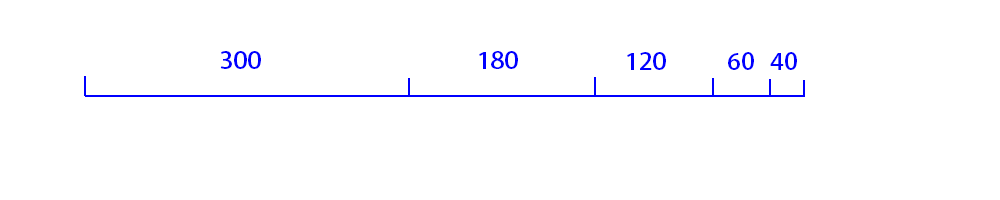
\includegraphics[width=0.5\textwidth]{./pics/Chapter_3/seikai_9.png}
            \end{figure}
        }
    \else
        \vspace{2cm}
    \fi
    % 2020华数之星初赛-三四年级真题.pdf ; 700
}

\item {
    【工程问题】
    甲乙两人合作加工一批零件, 如果甲先做10天, 乙再做8天就可以完成全部工作;如果甲先做6天, 乙再做16天也可以完成全部工作, 那么如果甲单独加工这批零件, \underline{\hbox to 20mm{}}天能完成全部工作.
    \ifshowSolution{}
        \fangsong\zihao{5}\textcolor{blue}{
            \\正解:\\
            设甲每天做x个,乙每天做y个.\\
            \[
                10x+8y = 6x+16y
            \]
            \[
                x= 2y
            \]
            假设甲每天做2个,则乙每天做1个,这批零件一共
            \[
                10x+8y = 28 个
            \]
            甲单独做,需要
            \[
                28\div 2 = 14天.
            \]
        }
    \else
        \vspace{2cm}
    \fi
    % 2020华数之星初赛-三四年级真题.pdf; 14
}

\item {
    【差倍问题】
    小花和小白一起去钓鱼, 若小花把自己钓的鱼给小白2条后, 小花剩下的鱼就是小白现在鱼数的4倍;若小花把自己钓的鱼给小白6条后, 小花剩下的鱼则是小白现在鱼数的2倍, 请问小花、小白各钓了几条鱼?
    \ifshowSolution{}
        \fangsong\zihao{5}\textcolor{blue}{
            \\正解:\\
            设小花x条,小白y条.\\
                \[\left\{\begin{array}{l}
                    x-2 = 4(y+2) \\
                    x-6 = 2(y+6)  
                \end{array}\right.\]
                \[\left\{\begin{array}{l}
                    x = 26 \\
                    y = 4 
                \end{array}\right.\]
        }
    \else
        \vspace{2cm}
    \fi
    % 2020华;26, 4
}

\item {
    【盈亏问题】
    六一儿童节, 老师给幼儿园大班的小朋友分水果, 已知苹果的总数是香蕉总数的 2 倍.如果给每个小朋友分3个香蕉, 就多出5个香蕉;每个小朋友分7个苹果, 就差两个苹果不够分, 那么大班共有\underline{\hbox to 20mm{}}个小朋友, 有\underline{\hbox to 20mm{}}个苹果.
    \ifshowSolution{}
        \fangsong\zihao{5}\textcolor{blue}{
            \\正解:\\
            设香蕉x个,则苹果2x个,人数为 $\frac{x-5}{3}$.\\
            \[
                2x + 2 = \frac{x-5}{3}\cdot 7
            \]
            \[
                x = 41, 
            \]
            \[
                \frac{x-5}{3} = 12
            \]
            所以,苹果有82个,有12个人.
        }
    \else
        \vspace{2cm}
    \fi
    % 2022 ; 华数真题2021-2023(小中组).pdf ; 
}

\item {
    【流水行船问题】
    一艘轮船,从上游A地开往下游B地,需要1小时,原路返程时,将船速提高到原来的2倍,也需要1小时. 那么,如果游轮从A地出发时也采用2倍船速,需要\underline{\hbox to 20mm{}}分钟可以到达B地.
    \ifshowSolution{}
        \fangsong\zihao{5}\textcolor{blue}{
            \\正解:\\
            $原船速度+水速 = 原船速\times 2 - 水速$\\
            $原船速=水速\times 2$\\
            游轮从A地出发时也采用2倍船速,则它的速度航行的速度是:
            \[原船速\times 2 + 水速 = 水速\times 5\]
            而原来从A地开往下游B地的航行速度是:
            \[原船速+水速 = 水速\times 3\]
            游轮从A地出发时也采用2倍船速与原来游轮从A地开往下游B地的速度比是:
            \[水速\times 5 : 水速\times 3 = 5:3\]
            \[60\times \frac35 = 36(分钟). \]
        }
    \else
        \vspace{2cm}
    \fi
    % 2014华, 36
}

\item {
    【不定方程整数解·枚举】
    赵老师出的新书有普通版和签名版两种版本, 普通版售价9元一本, 签名版售价 10 元一本.有一位顾客花 37 元买了若干本赵老师的新书, 那么其中有\underline{\hbox to 20mm{}}本签名版.
    \ifshowSolution{}
        \fangsong\zihao{5}\textcolor{blue}{
            \\正解:\\
            设普通版x本,签名版y本.\\
            \[9x + 10y = 37\]
            令$y=1, 2, 3$,得
            \[\left\{\begin{array}{l}
                    x = 3 \\
                    y = 1 
            \end{array}\right.\]
        }
    \else
        \vspace{2cm}
    \fi
    % 迎春杯三年级2022-试卷.pdf
}

\item {
    【年龄问题·位值原理】
    $2000\sim 2099$的某一年, 小高和爷爷正在聊天, 小高说:``爷爷, 我发现今年我的年龄正好是我出生年份的末两位.''爷爷想了想说:``巧了, 我也是.''如果爷爷的年龄正好是小高的3倍, 那么, 这一年是  \underline{\hbox to 20mm{}}年.(默认:年龄 = 这一年年份 - 出生年份)
    \ifshowSolution{}
        \fangsong\zihao{5}\textcolor{blue}{
            \\正解:\\
            设小高今年$\overline{AB}$岁,\\
            则今年的年份为$\overline{20AB} + \overline{AB}$, \\
            小高出生的年份为$\overline{20AB}$.\\
            爷爷的年龄为$30A + 3B$, 出生年份为$\overline{20AB} + \overline{AB} - 30A - 3B = 1900+100-10A-B$.\\
            \begin{align*}
                30A + 3B &= 100 - 10A- B \\
                即 10A + B &= 25, (其中A,B = 0,1,\ldots, 9)
            \end{align*}
            得
            \[ A=2, B=5 \]
            所以,今年是
            \[ 2025 + 25 = 2050. \]
        }
    \else
        \vspace{2cm}
    \fi
    % 迎春杯四年级2022-试卷.pdf ; 2050
}

\item {
    【等差数列应用题】
    某学校阶梯教室现有座位总数超过400个, 但不超过440个, 而且每一排都比前一排多两个座位, 若第一排只有12个座位, 这个阶梯教室一共有\underline{\hbox to 20mm{}}排座位.
    \ifshowSolution{}
        \fangsong\zihao{5}\textcolor{blue}{
            \\正解:\\
            设有n排座位.\\
            则第n排的座位数量:
            \[ 12+2(n-1) \]
            前n排的座位数量:
            \[ [12+12+2(n-1)]\cdot n \cdot \frac12 = n(n+11) \]
            当$n=16$时,
            \[ n(n+11) = 432. \]
        }
    \else
        \vspace{2cm}
    \fi
    % 2020华数之星初赛-三四年级真题.pdf; 16
}

%%%%%%%%%%%%%%%%%%%%%%%%%%%%%%%%%%%%%%%%%%%%
% \item {
%    【最优规则·周期】
%     某地7月的31天除了晴天就是雨天.有一颗新种的小树苗, 在每个晴天会长高3毫米, 在每个雨天会长高2毫米, 但连续经过6个晴天, 小树苗就会因为干旱而停止生长.那么整个7月小树苗最多长高\underline{\hbox to 20mm{}}毫米.
%     \vspace{2cm}
%     % 2024数学花园探秘笔试小中年级夏季决赛C卷(B5试卷版).pdf ; 88
% }

% \item {
%    【和倍问题】
%     小迎、小春、小杯三人分享 141颗巧克力:已知小杯分到的巧克力比小迎和小春分到的巧克力之和的两倍多6颗,小迎分到的巧克力比小春分到的巧克力的三倍少3颗.那么小迎分到\underline{\hbox to 20mm{}}颗巧克力.
%     \vspace{2cm}
%     % 2025;33
% }

% \item {
%     【不定方程】
%     红星小学围棋兴趣小组有4位小朋友和2位教练,4位小朋友依次相差2岁, 2位教练相台差2岁, 6个人年龄的平方和是2796岁, 6个人年龄之和是 \underline{\hbox to 20mm{}} 岁.
%     \vspace{2cm}
%     % 小高;2022年华数之星夏令营(广东营)答案解析.pdf;106
% }